\documentclass[a4paper,twoside]{book}

\emergencystretch=1em
\usepackage[utf8]{inputenc}
\usepackage[english]{babel}
\usepackage{fontspec}
\usepackage{graphicx}
\renewcommand{\thefigure}{\thesection.\arabic{figure}}
\usepackage{hyperref}
\usepackage{multirow}
\usepackage[absolute,overlay,showboxes]{textpos}
\usepackage{etoolbox}
\usepackage{longtable}
\usepackage{tikz}
\usepackage{lilyglyphs}
\usepackage{tabularx}
\usepackage{pgfplots}
\usepackage{circuitikz}
\usepackage{minted}
\usepackage{glossaries}
\usepackage{makeidx}
\usepackage{expl3}
\usepackage{chngcntr}
\usepackage{svg}
\usepackage{subfiles}
\usepackage[printonlyused,withpage]{acronym}

\usepackage[backend=bibtex]{biblatex}
\addbibresource{references.bib}

%%%%%%%%%%%%%%%%%%%%%%%%%%%%%%%%%%%%%%%%%%%%%%%%%%%%%%%%%%%%%%%%%%%%%%%%%%%%%%%%
\setmainfont{Liberation Serif}
\setmonofont{Liberation Mono}

\makeindex
\makeglossaries

\urlstyle{same}

\graphicspath{ {images/} {../../../images/} }

%% \documentclass[../main.tex]{subfiles}
%% \usepackage{svg}
%% \graphicspath{{\subfix{../images/}}}
%% \begin{document}

\newcounter{example-counter}
\setcounter{example-counter}{1}

%% This procedure adds the "Example" block to the text.
\newcommand{\example}[1]{
  \vspace{8pt}
  \begin{tabularx}{\textwidth}{m{1cm} m{9cm}}
    \includesvg[width=1.25cm]{the-noun-project/request-mirrored}
    & \textbf{Пример \arabic{example-counter}}: #1 \\
  \end{tabularx}
  \addtocounter{example-counter}{1}
}

\newcounter{experiment-counter}
\setcounter{experiment-counter}{1}

%% This procedure adds the "Experiment" block to the text.
\newcommand{\experiment}[2]{
  \vspace{8pt}
  \begin{tabularx}{\textwidth}{m{.15\textwidth}X m{.85\textwidth-4}X}
    \includesvg[width=1cm]{the-noun-project/flask}
    & \textbf{Эксперимент №\arabic{experiment-counter}:} #2 \\
  \end{tabularx}
  \addtocounter{experiment-counter}{1}
}

\newcommand{\note}[1]{
  \vspace{8pt}
  \begin{tabularx}{\textwidth}{m{1cm} m{9cm}}
    \includesvg[width=1cm]{the-noun-project/note}
    & \textbf{Примечание:} #1 \\
  \end{tabularx}
}

\newcommand{\hotkey}[1]{
  \texttt{#1}
}

%% This procedure allows to insert a music note.
%% Syntax:
%%   \musicnote{<octave>}{<note-name>}{<frequency>}
\newcommand{\musicnote}[3]{
  &
  \ifstrequal{#2}{C}{До   & C#1}{}
  \ifstrequal{#2}{D}{Ре   & D#1}{}
  \ifstrequal{#2}{E}{Ми   & E#1}{}
  \ifstrequal{#2}{F}{Фа   & F#1}{}
  \ifstrequal{#2}{G}{Соль & G#1}{}
  \ifstrequal{#2}{A}{Ля   & A#1}{}
  \ifstrequal{#2}{B}{Си   & B#1 (H#1)}{}
  & #3 \\
}

%% Taken from:
%%   <https://tex.stackexchange.com/questions/184923/how-to-include-a-second-file-only-if-environment-variable-is-set>
\newcommand{\newgetenv}[2][]{%
 \CatchFileEdef{\temp}{"|kpsewhich --var-value #2"}{\endlinechar=-1\relax}%
 \if\relax\detokenize{#1}\relax\temp\else\edef#1{\temp}\fi%
}%

\newcommand\esymbol[1]{%
  \begin{circuitikz}%
    \draw (0,0) to [#1] (1,0);%
  \end{circuitikz}%
}

\newcommand*{\soundWaveIcon}[0]{%
  
\begin{tikzpicture}
    \draw[black, fill=black] (0, 0) circle (.25mm);
    \draw (.5mm, 0.7mm) arc (45:-45:1mm);
    \draw (1mm, 1mm) arc (45:-45:1.5mm);
    \draw (1.5mm, 1.3mm) arc (45:-45:2mm);
  \end{tikzpicture}%
}

%% \end{document}

\newcommand{\figureSoundGraph}[1]{
  \begin{figure}[H]
    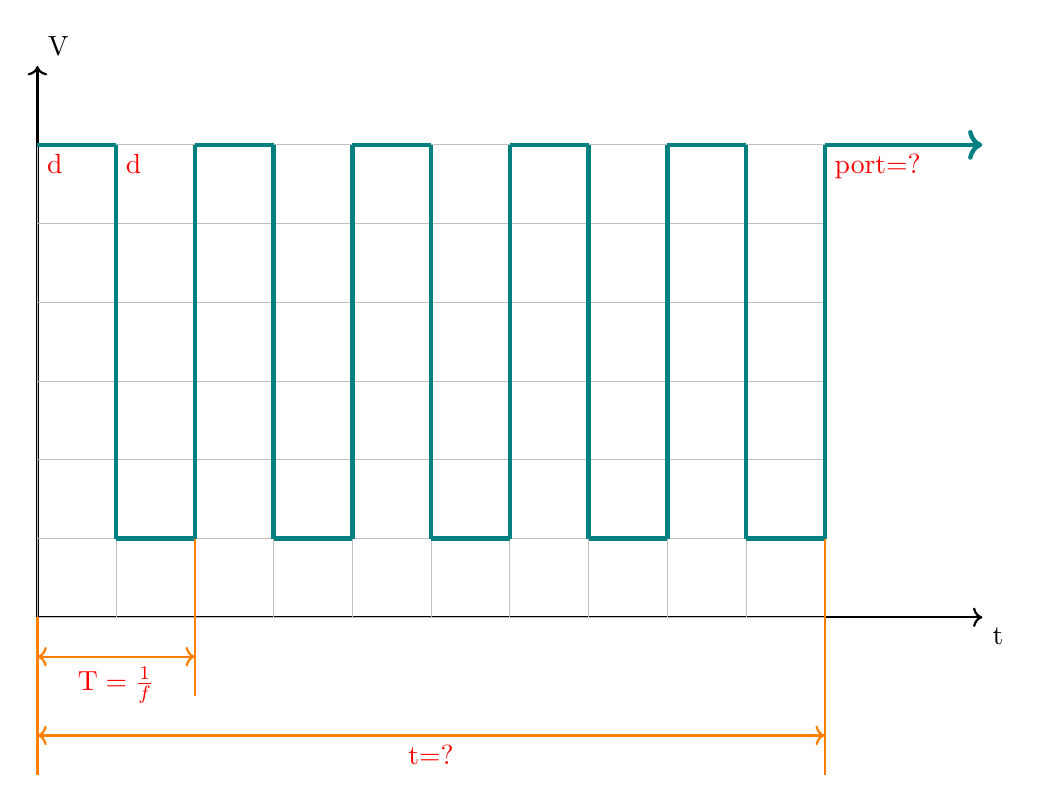
\begin{tikzpicture}
      \draw[thick, ->] (0, 0) -- (12, 0) node[anchor=north west] {t};
      \draw[thick, ->] (0, 0) -- (0,  7) node[anchor=south west] {V};
      \draw[lightgray] (0, 0) grid (10, 6);
      \foreach \x in {0, 2, ..., 8} {
        \draw[ultra thick, teal] (\x, 6) -- (\x + 1, 6);
        \draw[ultra thick, teal] (\x + 1, 6) -- (\x + 1, 1);
        \draw[ultra thick, teal] (\x + 1, 1) -- (\x + 2, 1);
        \draw[ultra thick, teal] (\x + 2, 1) -- (\x + 2, 6);
      }
      \draw[ultra thick, teal, ->] (10, 6) -- (12, 6);
      \draw[orange] (10, 6) node[anchor=north west, red] {port=?};
      \draw[orange] (0, 6) node[anchor=north west, red] {d};
      \draw[orange] (1, 6) node[anchor=north west, red] {d};
      \draw[thick, orange] (0,  0) -- (0,   -2);
      \draw[thick, orange] (2,  1) -- (2,   -1);
      \draw[thick, orange] (10, 1) -- (10,  -2);
      \draw[thick, orange, <->] (0, -0.5)
      -- (2,  -0.5) node[midway, below, red] {$\mbox{T} = \frac{1}{f}$};
      \draw[thick, orange, <->] (0, -1.5)
      -- (10,  -1.5) node[midway, below, red] {t=?};
    \end{tikzpicture}
    \caption{#1}
    \label{fig:sound-graph}
  \end{figure}
}


\counterwithin{listing}{section}

\newgetenv[\REPRODUCIBILITY]{REPRODUCIBILITY}%
\newgetenv[\RANDOMSEED]{RANDOMSEED}

\ifdefstring{\REPRODUCIBILITY}{yes}{%
  \ifthenelse{\equal{\RANDOMSEED}{}}%
  {%
    \typeout{Setting the random seed to a fixed value.}%
    \pgfmathsetseed{\number42}%
  }{%
    \typeout{Setting the random seed to a \RANDOMSEED .}%
    \pgfmathsetseed{\number\RANDOMSEED}%
  }%
}{}

%%%%%%%%%%%%%%%%%%%%%%%%%%%%%%%%%%%%%%%%%%%%%%%%%%%%%%%%%%%%%%%%%%%%%%%%%%%%%%%%
\title{Science, Programming, Art and Radioelectronics Club\\(SPARC)}
\author{Artyom ``avp'' Poptsov\\\href{https://memory-heap.org}{memory-heap.org}}
\input{out/src/en/version.tex}

\begin{document}

\maketitle

\tableofcontents

%%%%%%%%%%%%%%%%%%%%%%%%%%%%%%%%%%%%%%%%%%%%%%%%%%%%%%%%%%%%%%%%%%%%%%%%%%%%%%%%
\chapter*{Introduction}
\addcontentsline{toc}{chapter}{Introduction}

%% TODO:

\subfile{sections/introduction.tex}

%%%%%%%%%%%%%%%%%%%%%%%%%%%%%%%%%%%%%%%%%%%%%%%%%%%%%%%%%%%%%%%%%%%%%%%%%%%%%%%%
\chapter{Electronics}
\label{chapter:electronics}

%% TODO:
\subfile{sections/electronics-introduction.tex}
\subfile{sections/electronics-voltage}
\subfile{sections/electronics-circuits.tex}
\subfile{sections/electronics-potential-difference}
\subfile{sections/electronics-resistance}
\subfile{sections/electronics-building-circuits}

%%%%%%%%%%%%%%%%%%%%%%%%%%%%%%%%%%%%%%%%%%%%%%%%%%%%%%%%%%%%%%%%%%%%%%%%%%%%%%%%
\chapter{Dialogues with a Computer}
\label{chapter:dialogues-with-computer}

\subfile{sections/dialogues-with-computer-title-image}
\subfile{sections/dialogues-with-computer-introduction}
\subfile{sections/dialogues-with-computer-algorithms}
\subfile{sections/dialogues-with-computer-arduino}
\subfile{sections/dialogues-with-computer-breadboard}
\subfile{sections/dialogues-with-computer-multimeter}

\newpage
\subfile{sections/dialogues-with-computer-arduino-ide}
\subfile{sections/dialogues-with-computer-program-structure}
\subfile{sections/dialogues-with-computer-memory}
\subfile{sections/dialogues-with-computer-control-flow}
\subfile{sections/dialogues-with-computer-wokwi}

%%%%%%%%%%%%%%%%%%%%%%%%%%%%%%%%%%%%%%%%%%%%%%%%%%%%%%%%%%%%%%%%%%%%%%%%%%%%%%%%
\chapter{White noise}
\label{chapter:white-noise}

\subfile{sections/white-noise-introduction}
\subfile{sections/white-noise-signal-types}
\subfile{sections/white-noise-serial-port}
\subfile{sections/white-noise-analog-ports}
\subfile{sections/white-noise-adc}

%%%%%%%%%%%%%%%%%%%%%%%%%%%%%%%%%%%%%%%%%%%%%%%%%%%%%%%%%%%%%%%%%%%%%%%%%%%%%%%%
\chapter{Pulse-Width Modulation}
\label{chapter:pwm}

\subfile{sections/pwm-intro}
\subfile{sections/pwm-wavelength}
\subfile{sections/pwm-duty-cycle}
\subfile{sections/pwm-tasks}

%%%%%%%%%%%%%%%%%%%%%%%%%%%%%%%%%%%%%%%%%%%%%%%%%%%%%%%%%%%%%%%%%%%%%%%%%%%%%%%%
\chapter{Music and Technology Synthesis}
\label{chapter:music-and-technology-synthesis}

\subfile{sections/music-and-technology-synthesis-sound}
\subfile{sections/music-and-technology-synthesis-speaker}
\subfile{sections/music-and-technology-synthesis-rhythm}
\subfile{sections/music-and-technology-synthesis-harmony}
\subfile{sections/music-and-technology-synthesis-octave-system}
\subfile{sections/music-and-technology-synthesis-simple-melodies}
\subfile{sections/music-and-technology-synthesis-arrays}
\subfile{sections/music-and-technology-synthesis-two-dimensional-arrays}
\subfile{sections/music-and-technology-synthesis-staff}
\subfile{sections/music-and-technology-synthesis-rest}
\subfile{sections/music-and-technology-synthesis-dotted-notes}
\subfile{sections/music-and-technology-synthesis-flats-and-sharps}
\subfile{sections/music-and-technology-synthesis-time-signature}
\subfile{sections/music-and-technology-synthesis-bass-clef}
\subfile{sections/music-and-technology-synthesis-music-band}

%%%%%%%%%%%%%%%%%%%%%%%%%%%%%%%%%%%%%%%%%%%%%%%%%%%%%%%%%%%%%%%%%%%%%%%%%%%%%%%%
%% \chapter{Computer Language}
%% \label{chapter:computer-language}

%% TODO:

%%%%%%%%%%%%%%%%%%%%%%%%%%%%%%%%%%%%%%%%%%%%%%%%%%%%%%%%%%%%%%%%%%%%%%%%%%%%%%%%
%% \chapter{Game Development}
%% \label{chapter:game-development}

%% TODO:

%%%%%%%%%%%%%%%%%%%%%%%%%%%%%%%%%%%%%%%%%%%%%%%%%%%%%%%%%%%%%%%%%%%%%%%%%%%%%%%%
\addcontentsline{toc}{chapter}{Index}
\printindex

%%%%%%%%%%%%%%%%%%%%%%%%%%%%%%%%%%%%%%%%%%%%%%%%%%%%%%%%%%%%%%%%%%%%%%%%%%%%%%%%
\addcontentsline{toc}{chapter}{Glossary}
\printglossaries

%%%%%%%%%%%%%%%%%%%%%%%%%%%%%%%%%%%%%%%%%%%%%%%%%%%%%%%%%%%%%%%%%%%%%%%%%%%%%%%%
\addcontentsline{toc}{chapter}{Code listings}
\renewcommand\listoflistingscaption{Code listings}
\listoflistings

%%%%%%%%%%%%%%%%%%%%%%%%%%%%%%%%%%%%%%%%%%%%%%%%%%%%%%%%%%%%%%%%%%%%%%%%%%%%%%%%
\printbibliography[heading=bibintoc, title={Bibliography}]

%%%%%%%%%%%%%%%%%%%%%%%%%%%%%%%%%%%%%%%%%%%%%%%%%%%%%%%%%%%%%%%%%%%%%%%%%%%%%%%%
\appendix

\subfile{sections/appendix-octaves}
\subfile{sections/appendix-prostokvashino-score}
\subfile{sections/appendix-twinkle-twinkle-little-star-01}
\subfile{sections/appendix-twinkle-twinkle-little-star-02}

\end{document}
